\documentclass[../main.tex]{subfiles} % Due to use of package subfiles

%%%%%%%%%%%%%%%%%%%%%%%%%%%%%%%%%%%%%%%%%%%%%%%%%%%%%%%%%%%%%%%%%%%%%%%%%%%%%%%%

\begin{document}

% \chapter{Lattice Schwinger Model and Confinement} \label{chap:Confinement}
\chapter{Confinement in the Lattice Schwinger Model} \label{chap:Confinement}

\ldots



% \section{Confinement and string breaking}
\section{QED, QCD, and confinement} \label{sec:Confinement}

\lipsum[1-3]


%%%%%

\begin{figure}[t]
    \centering
    \begin{tikzpicture}
        % Include the image
        \node[anchor=south west, inner sep=0] (image) at (0, 0) {
            \ifthenelse{\boolean{book}}{
                % Image remains the same size in book as in report class
                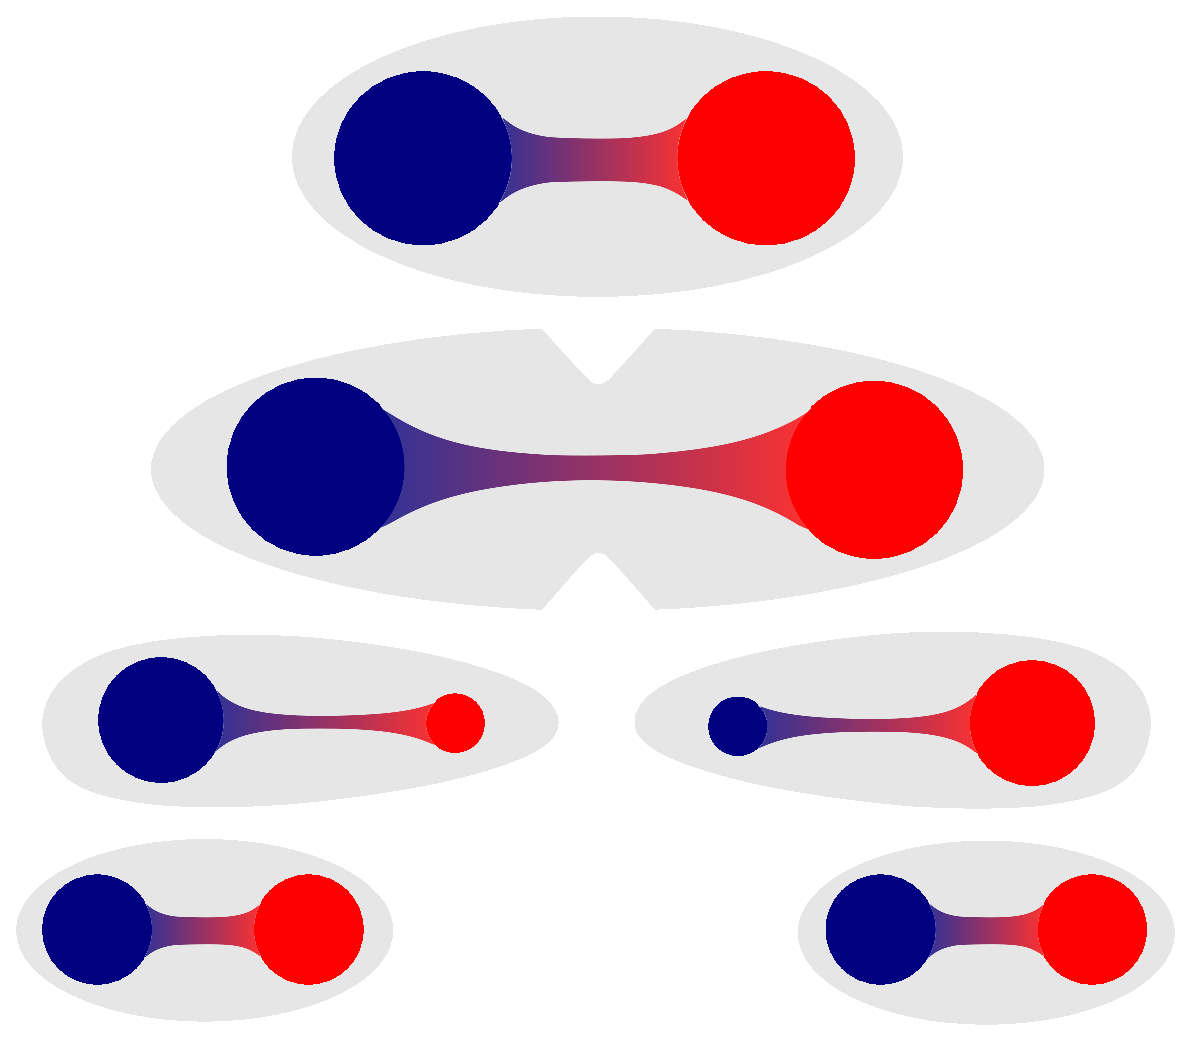
\includegraphics[width=0.7\textwidth]{images/QuarkConfinement.eps}
            }{
                % Size of image in report class
                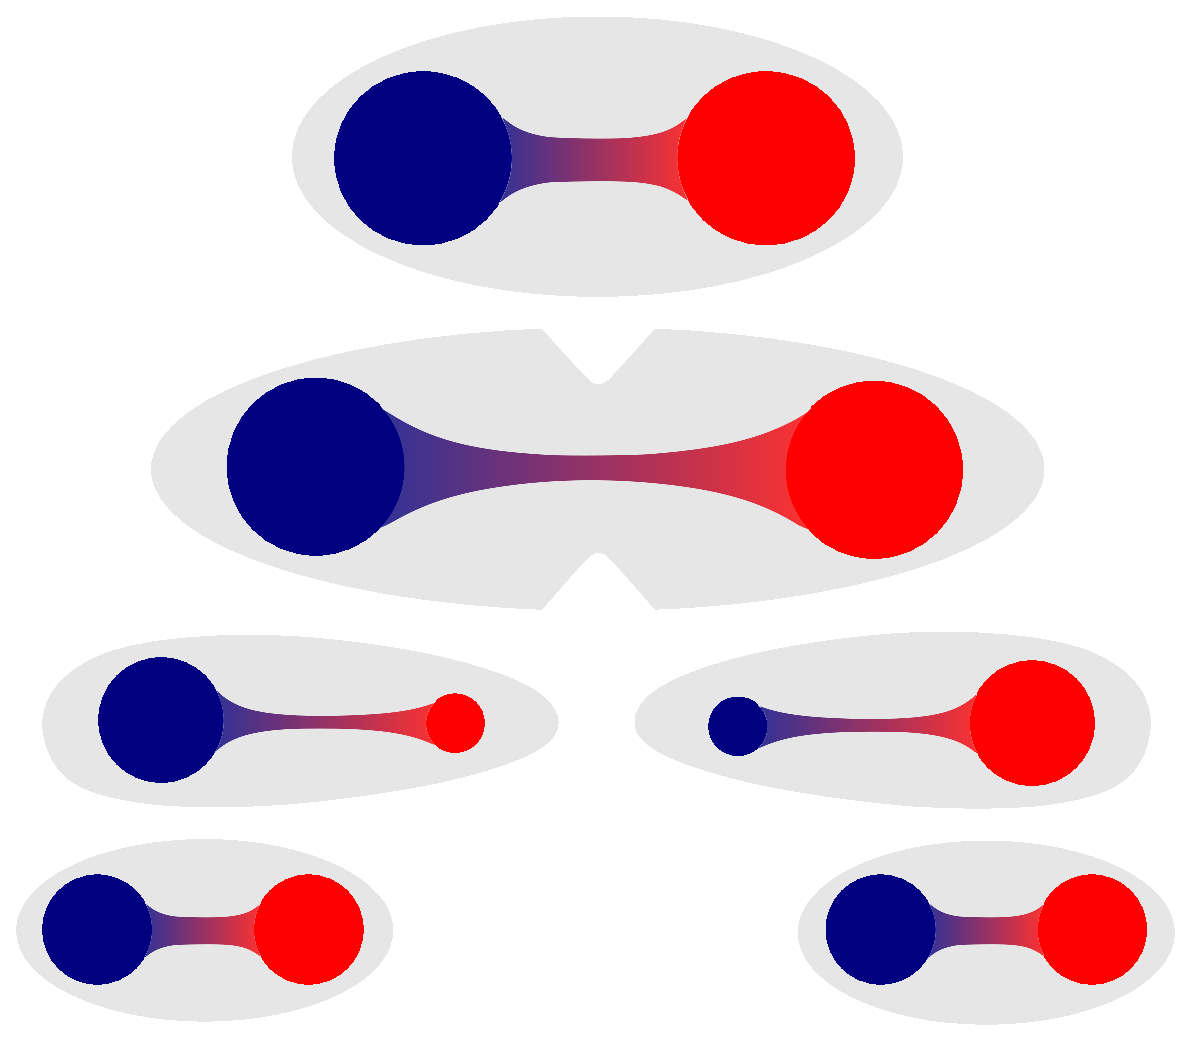
\includegraphics[width=0.8\textwidth]{images/QuarkConfinement.eps}
            }
        };
        % Draw the coordinate system
        \begin{scope}[x={(image.south east)},y={(image.north west)}]
            \draw[thick,|-|] (0.35, 1.03) -- node[above, midway] {\large $r$} (0.65, 1.03);
            \draw[thick,->] (0, 1) -- node[right, midway] {\large time} (0, 0.8);
        \end{scope}
    \end{tikzpicture}
    \caption{As a quark\index{quark} (red) and an antiquark\index{antiquark} (blue) in a meson\index{meson} are pulled away from each other (distance $r$ increases), the energy needed increases until the string tension of the flux tube\index{flux tube} (blue to red gradient) between the particles is sufficient enough, thus the flux tube break, known as string breaking\index{string breaking}, and the energy stored in the flux tube creates a new quark and antiquark such that there is now two mesons. That a quark and an antiquark can never exist on its own is know as colour confinement\index{colour confinement}\index{confinement|see{colour confinement}}. Inspired by Ref. \cite{institutoDeFisicaCorpuscular_numericalApproach_2016}.}
    \label{fig:QuarkConfinement}
\end{figure}

%%%%%



\section{Lattice Schwinger model exhibiting confinement} \label{sec:LatticeSchwingerModelAndConfienemt}

\ldots

\cref{eq:LatticeSchwingerModelHamiltonianSpin}
\begin{align}
    H &= a \sum_n \left[ (-1)^{n+1} \frac{m}{2} \sigma_n^z - \frac{1}{2a} \left( \sigma_n^+ S_n^+ \sigma_{n+1}^- + \mathrm{h.c.} \right) + \frac{a^2 q^2 S^2}{2} \left( S_n^z \right)^2 \right]
\end{align}



\subsection{Computing the states} \label{sec:StateComputing}

\ldots

\cref{eq:GeneratorU(1)SymmetryDiscretized} changes to become
\begin{align}
    G_n = \frac{E_n - E_{n-1}}{a} - q \psi_n\dagger \psi_n - \frac{(-1)^n - 1}{2} \: ,
\end{align}
\begin{align} \label{eq:GeneratorU(1)Symmetry}
    G_n = - S_n^z + S_{n-1}^z - \frac{q}{2} \big( - \sigma_n + (-1)^n \big) \: ,
\end{align}
for $S=1$. \cite{buyens_confinementAndStringBreaking_2016}

\begin{table}[t]
    \centering
    \begin{tabular}{|c|c|c|}
        \hline
        State & \multicolumn{2}{c|}{$G_n / q$} \\
         & Even $n$ & Odd $n$ \\ \hline
        $\ket{\, 0_g\, 0_m\, 0_g}$ & $0$ & $1$ \\ \hline
        $\ket{\, 0_g\, 1_m\, 0_g}$ & $-1$ & $0$ \\ \hline
        $\ket{\, 0_g\, 0_m\, 1_g}$ & $1$ & $2$ \\ \hline
        $\ket{\, 0_g\, 1_m\, 1_g}$ & $0$ & $1$ \\ \hline
        $\ket{\, 0_g\, 0_m\, 2_g}$ & $2$ & $3$ \\ \hline
        $\ket{\, 0_g\, 1_m\, 2_g}$ & $1$ & $2$ \\ \hline
        $\ket{\, 1_g\, 0_m\, 0_g}$ & $-1$ & $0$ \\ \hline
        $\ket{\, 1_g\, 1_m\, 0_g}$ & $-2$ & $-1$ \\ \hline
        $\ket{\, 1_g\, 0_m\, 1_g}$ & $0$ & $1$ \\ \hline
        \multicolumn{3}{|c|}{\textsl{continued to the right}} \\ \hline
    \end{tabular}
    \hfill
    \begin{tabular}{|c|c|c|}
        \hline
        State & \multicolumn{2}{c|}{$G_n / q$} \\
         & Even $n$ & Odd $n$ \\ \hline
        \multicolumn{3}{|c|}{\textsl{continued from the left}} \\ \hline
        $\ket{\, 1_g\, 1_m\, 1_g}$ & $-1$ & $0$ \\ \hline
        $\ket{\, 1_g\, 0_m\, 2_g}$ & $1$ & $2$ \\ \hline
        $\ket{\, 1_g\, 1_m\, 2_g}$ & $0$ & $1$ \\ \hline
        $\ket{\, 2_g\, 0_m\, 0_g}$ & $-2$ & $-1$ \\ \hline
        $\ket{\, 2_g\, 1_m\, 0_g}$ & $-3$ & $-2$ \\ \hline
        $\ket{\, 2_g\, 0_m\, 1_g}$ & $-1$ & $0$ \\ \hline
        $\ket{\, 2_g\, 1_m\, 1_g}$ & $-2$ & $-1$ \\ \hline
        $\ket{\, 2_g\, 0_m\, 2_g}$ & $0$ & $1$ \\ \hline
        $\ket{\, 2_g\, 1_m\, 2_g}$ & $-1$ & $0$ \\ \hline
    \end{tabular}
    \caption{The eigenvalues of the generator from \cref{eq:GeneratorU(1)Symmetry} for the 18 configurations of two gauge fields (denoted with a $g$) with spin-$1$ and the matter field (denoted with an $m$) with spin-\half between them.}
    \label{tab:EigenvaluesOfGenerator}
\end{table}



\subsection{Confinement and string breaking} \label{sec:ConfienementAndStringBreakingAnalyticalAndNumerical}

\subsubsection{Analytical results}

\ldots



\subsubsection{Numerical results}

\ldots

\begin{figure}[t]
    \centering
    \begin{tikzpicture}[
        % Definition of node styles
        particle/.style={circle, fill=red!100, very thick, minimum size=2mm},
        antiparticle/.style={circle, fill=blue!100, very thick, minimum size=2mm},
        node distance = 1.75cm,
        emptysite/.style={circle, draw=black!40, minimum size=2mm},
        node distance = 1.75cm,
        ]
        %
        % Nodes
        \node[label={[label distance=.3cm]above:{\large $E_n$ direction}}, label={[label distance=.3cm]below:{\large Site number}}] (text) {\large Configuration};
        \node[antiparticle, label={[label distance=.5cm]below:{\large $1$}}] (firstParticle) [right=.5cm of text] {};
        \node[emptysite, label={[label distance=.5cm]below:{\large $2$}}] (firstAntiparticle) [right=of firstParticle] {};
        \node[emptysite, label={[label distance=.5cm]below:{\large $3$}}] (secondParticle) [right=of firstAntiparticle] {};
        \node[particle, label={[label distance=.5cm]below:{\large $4$}}] (secondAntiparticle) [right=of secondParticle] {};
        %
        % Links
        \draw[dashed] (firstParticle.east) -- node[above=0.75cm, midway, black] {\Large $\leftarrow$} (firstAntiparticle.center);
        \draw[dashed] (firstAntiparticle.center) -- node[above=0.75cm, midway, black] {\Large $\leftarrow$} (secondParticle.center);
        \draw[dashed] (secondParticle.center) --  node[above=0.75cm, midway, black] {\Large $\leftarrow$} (secondAntiparticle.west);
        %
        % Name of the state
        \node at (-1,2) {\large \underline{State $\varphi$}};
    \end{tikzpicture}
    \newline
    \vspace{.4em}
    \begin{tikzpicture}[
        % Definition of node styles
        particle/.style={circle, fill=red!100, very thick, minimum size=2mm},
        antiparticle/.style={circle, fill=blue!100, very thick, minimum size=2mm},
        node distance = 1.75cm,
        ]
        %
        % Nodes
        \node[label={[label distance=.3cm]above:{\large $E_n$ direction}}, label={[label distance=.3cm]below:{\large Site number}}] (text) {\large Configuration};
        \node[antiparticle, label={[label distance=.5cm]below:{\large $1$}}] (firstParticle) [right=.5cm of text] {};
        \node[particle, label={[label distance=.5cm]below:{\large $2$}}] (firstAntiparticle) [right=of firstParticle] {};
        \node[antiparticle, label={[label distance=.5cm]below:{\large $3$}}] (secondParticle) [right=of firstAntiparticle] {};
        \node[particle, label={[label distance=.5cm]below:{\large $4$}}] (secondAntiparticle) [right=of secondParticle] {};
        %
        % Links
        \draw[dashed] (firstParticle.east) -- node[above=0.75cm, midway, black] {\Large $\leftarrow$} (firstAntiparticle.west);
        \draw[dashed, black!40] (firstAntiparticle.east) -- node[above=0.75cm, midway, black] {\Large $0$} (secondParticle.west);
        \draw[dashed] (secondParticle.east) --  node[above=0.75cm, midway, black] {\Large $\leftarrow$} (secondAntiparticle.west);
        %
        % Name of the state
        \node at (-1,2) {\large \underline{State $\chi$}};
    \end{tikzpicture}
    \caption{The two states for which the numerical study of string breaking is performed. The system starts in state $\varphi$ with the variables set to be favourable for string breaking, thus the system will over time go to state $\chi$. The red and blue circles are quarks and antiquarks respectively, the grey outlined circles are sites with neither a quark nor an antiquark, and the dashed lines is the gauge field (electric field). The direction of the electric field between the quarks and antiquarks is noted above the lattice links, and the grey dashed line reflects the electric field not being present.}
    \label{fig:SystemForNumericalSimulationOfConfinementAndStringBreaking}
\end{figure}




\section{Outlook} \label{sec:Outlook}

\ldots




\end{document}